\documentclass[11pt,a4paper]{report}

% Aberstwyth dissertation LaTeX Template
% Authors: Dr. Hannah Dee (hmd1@aber.ac.uk), Neil Taylor (nst@aber.ac.uk)
% This has been adapted from the Leeds Thesis template and the
% Group Project template for Computer Science in Aberystywth University.
%
% All comments and suggestions welcome.
%
% Template designed to be used with pdflatex: it may need alteration to
% run with a different LaTeX engine

% To build document on the unix command line, run four commands:

% pdflatex dissertation
% bibtex dissertation
% pdflatex dissertation
% pdflatex dissertation

% you will end up with dissertation.pdf
\usepackage{mmp}

% the following packages are used for citations - You only need to include one.
%
% Use the cite package if you are using the numeric style (e.g. IEEEannot).
% Use the natbib package if you are using the author-date style (e.g. authordate2annot).
% Only use one of these and comment out the other one.
\usepackage{cite}
%\usepackage{natbib}

% Use the following to selectively exclude chapters
%\includeonly{cover,abstract,acknowledge,declare,chapter1,chapter2}

\begin{document}

% all of the include directives below refer to tex files
% so %TC:ignore
\title{Can entropy-based image alignment metrics offer improved image aggregation of tissue density for mammographic risk assessment?}

% Your name
\author{Laura Collins}

% Your email
\authoremail{lac32@aber.ac.uk}

\degreeschemecode{GH7P} %e.g. G400
\degreeschemetitle{Artificial Intelligence and Robotics (inc Integrated Industrial and Professional Training)} % e.g. Computer Science
\degreetype{BSc}

\modulecode{CS39440} % i.e. CS39440, CC39440, CS39620
\moduletitle{Major Project} % i.e. Major Project or Minor Project

\date{4th March 2016} % i.e. the date of this version of the report

\status{Draft} % Use draft until you create the release version. Then, change this to Release.
\version{1.0}

%The title and name of your supervisor.
\supervisor{Dr. Neil Mac Parthal\'ain}

%The email for your supervisor.
\supervisoremail{ncm@aber.ac.uk}

\maketitle

%TC:endignore
 includes cover.tex - to change the content,
% edit the tex file

\pagenumbering{roman}

% This is the front page
%TC:ignore
\title{Can entropy-based image alignment metrics offer improved image aggregation of tissue density for mammographic risk assessment?}

% Your name
\author{Laura Collins}

% Your email
\authoremail{lac32@aber.ac.uk}

\degreeschemecode{GH7P} %e.g. G400
\degreeschemetitle{Artificial Intelligence and Robotics (inc Integrated Industrial and Professional Training)} % e.g. Computer Science
\degreetype{BSc}

\modulecode{CS39440} % i.e. CS39440, CC39440, CS39620
\moduletitle{Major Project} % i.e. Major Project or Minor Project

\date{4th March 2016} % i.e. the date of this version of the report

\status{Draft} % Use draft until you create the release version. Then, change this to Release.
\version{1.0}

%The title and name of your supervisor.
\supervisor{Dr. Neil Mac Parthal\'ain}

%The email for your supervisor.
\supervisoremail{ncm@aber.ac.uk}

\maketitle

%TC:endignore


% Set up page numbering
\pagestyle{empty}

% declarations of originality
\thispagestyle{empty}

%%%
%%% You must sign the declaration of originality. 
%%%
\begin{center}
    {\LARGE\bf Declaration of originality}
\end{center}

In signing below, I confirm that:

\begin{itemize}
\item{This submission is my own work, except where 
clearly indicated.}

\item{I understand that there are severe penalties for 
Unacceptable Academic Practice, which can lead to loss 
of marks or even the withholding of a degree.}
 
\item{I have read the regulations on Unacceptable Academic 
Practice from the University's Academic Quality and 
Records Office (AQRO) and the relevant sections of the 
current Student Handbook of the Department of 
Computer Science.}
 
\item{In submitting this work I understand and agree to 
abide by the University's regulations governing these issues.}
\end{itemize}

\vspace{2em}
Name ............................................................  \\

\vspace{1em}
Date ............................................................ \\

%%% 
%%% We would like to make a selection of final reports available to students that take 
%%% this module in future years. To enable us to do this, we require your consent. You 
%%% are not required that you do this, but if you do give your consent, then we will have 
%%% the option to select yours as one of a number of reports as examples for other 
%%% students. If you would like to give your consent, then please include the following 
%%% text and sign below. If you do not wish to give your consent, please remove this 
%%% from your report. 
%%%
\vspace{1em}
\begin{center}
    {\LARGE\bf Consent to share this work}
\end{center}

In signing below, I hereby agree to this dissertation being made available to other
students and academic staff of the Aberystwyth Computer Science Department.  

\vspace{2em}
Name ............................................................  \\

\vspace{1em}
Date ............................................................ \\




\thispagestyle{empty}

\begin{center}
    {\LARGE\bf Acknowledgements}
\end{center}

I would like to thank my Supervisor Neil for his constant help and guidance throughout this project.
 % Acknowledgements
\thispagestyle{empty}

\begin{center}
    {\LARGE\bf Abstract}
\end{center}

This project will assess whether leveraging image alignment techniques to align mammographic images using fuzzy entropy and shannon entropy metrics will produce a sensible output. This output could then aid Mammographers in the classification a patient's breast tissue density.
                 % Abstract

\pagenumbering{roman}
\pagestyle{fancy}
\fancyhead{}
\fancyfoot[C]{\thepage}
\renewcommand{\headrulewidth}{0 pt}
\renewcommand{\chaptermark}[1]{\markboth{#1}{}}

\tableofcontents
\newpage
\listoffigures
\newpage
\listoftables
\newpage

% Set up page numbering
\pagenumbering{arabic}

\setchapterheaderfooter

% include the chapters
\chapter{Background \& Objectives}

\section{Project Description}
The Project is concerned with the alignment of multiple images using an image-alignment technique called Congealing \cite{joint-alignment}. The paper describes a method which utilises the Congealing algorithm to align both MNIST handwriting data and MRI Scans by reducing the pixel-wise uncertainty across a collection of images. This project aims to go further, aligning mammography scans and reducing the pixel-wise uncertainty using a number of different fuzzy entropy methods.

\section{Research Method}

%You need to describe briefly the life cycle model or research method that you used. You do not need to write about all of the different process models that you are aware of. Focus on the process model or research method that you have used. It is possible that you needed to adapt an existing method to suit your project; clearly identify what you used and how you adapted it for your needs.

For this project, a literature review was undertaken to assess the work completed by researchers in the fields of Entropy, Fuzzy Entropy and image alignment methods to help better understand what has been investigated, and to gain an understanding of the background.

\subsection{Entropy}
\label{ssec:entropy}

In terms of Information Theory, the Merriam-Webster Dictionary defines Entropy to be \cite{def_entropy}:

\begin{quotation}
 \textit{Entropy (noun): the degree of disorder or uncertainty in a system}
\end{quotation}

Shannon entropy, derived by Claude Shannon \cite{shannon1948a} can be mathematically defined as :

\begin{equation}
  H(X) = - \displaystyle\sum_{i=0}^{N}{p_i \log_2 p_i}
\end{equation}
\myequations{Shannon Entropy}

Where $p_i$ is the set of probabilities for all the variables in $X$.

Let us consider a fair coin toss. The probability of heads is exactly $\frac{1}{2}$, therefore, the entropy of landing on heads is:

\begin{equation}
  \begin{split}
    H(heads) &= -\frac{1}{2}\log_2(\frac{1}{2}) - \frac{1}{2}\log_2(\frac{1}{2}) \\
    &= 1.0
  \end{split}
\end{equation}
\myequations{Shannon Entropy example - coin toss}

On the other side, if a system outputs solely the letter \say{M}, then the entropy of receiving the letter \say{M} is exactly 0. This is because when either the positive or the negative outcome is 100\%, then both sides equal \say{0} when fed into the entropy equation.
%http://mirror.ox.ac.uk/sites/ctan.org/graphics/pgf/contrib/pgfplots/doc/pgfplots.pdf
\begin{figure}[H]
  \iffalse
\begin{center}
\pgfplotsset{every axis/.append style={thick},width=0.4*\textwidth, ymax=1}
\begin{tikzpicture}
 \begin{axis}[
     axis lines = left,
    xlabel = $p$,
    ylabel = {Entropy},
    ]
  \addplot [
    domain=-0:1,
    samples=100,
    color=cyan,
    ]
    { -( x * log2(x) + (1-x) * log2(1-x) )};
  \end{axis}
\end{tikzpicture}
\end{center}
\caption{Entropy mapped against probability ($p$) of occurrence.}
\label{fig:entropy}
\fi
\end{figure}

It follows that entropy can only ever take a value between 0 and 1, with an entropy of 1 have a 50\% probability, and an entropy of 0 being 100\% certain.

\subsection{Uncertainty}

However real life is not 100\% certain - a small amount of uncertainty in life is to be expected and sometimes desired. A surprise party for many is the nice kind, however uncertainty associated with risk - i.e. \say{Will I lose my job in the recession?} - is uncertainty with a negative impact. Modeling uncertainty is especially important to researchers so they can understand it, and use it to our advantage in techniques such as fuzzy entropy.

\subsubsection{Probabilistic Uncertainty}

By definition:

\begin{quotation}
  \textit{Probability: the chance that something will happen \cite{PROBABILITY}}
\end{quotation}

Probabilistic distribution is a widely accepted and used technique for representing expert judgements of uncertainty \cite{O’Hagan_2011}. Early work carried out by DeGroot (1970) \cite{degroot2004optimal}, built upon that of Savage (1954) \cite{Savage_1954}, gave a simple layman's explanation:

\begin{quotation}
  \textit{For instance, if the person prefers decision A to B and B to C then they must also prefer A to C.}
\end{quotation}

\subsubsection{Possibilistic Uncertainty}

By definition:

\begin{quotation}
  \textit{Possibility: a chance that something might exist, happen, or be true : the state or fact of being possible \cite{POSSIBILITY}}
\end{quotation}

Possibilistic uncertainty (closely related to \say{fuzziness}) indicates the lack of information we hold about the possible outcome values from a system - a sort of ambiguity. Possibilistic uncertainty models the possible outcomes from a system, as estimated by a decision maker because it is possibly impossible to determine beforehand \cite{Untiedt_2010}.

\subsubsection{Indiscernibility Uncertainty}

By definition:

\begin{quotation}
  \textit{Indiscernibility: the quality or state of being indiscernible \cite{INDISCERNIBILITY}}

  \textit{Indiscernible: impossible to see, hear, or know clearly \cite{INDISCERNIBLE}}
\end{quotation}

\todo[inline]{Find an explanation of Indiscernibility}


\subsection{Fuzzy Entropy}
\label{ssec:fuzzy-entropy}

Fuzzy entropy stems from combining standard Shannon entropy with the practices of Fuzzy Set Theory, discovered by Zadeh in 1965 \cite{Zadeh_1965}. This introduces the idea of \say{Membership} to a category, where an object can belong to more than one category to a certain degree.

One common example of this is listing someone as `Short', `Average' or `Tall' in height. If a tall person is someone over 6 feet in height, would a person who measured 5foot 11inches not be classified as tall? Given crisp sets, then they would be classified as `Average'. In fuzzy set theory, they would be be a certain degree of tall, and a certain degree of average, with the highest membership likely to win out when categorising their height. Another example of this can be seen in Figure \ref{fig:fuzzy-sets}

\begin{figure}[H]
  \center
  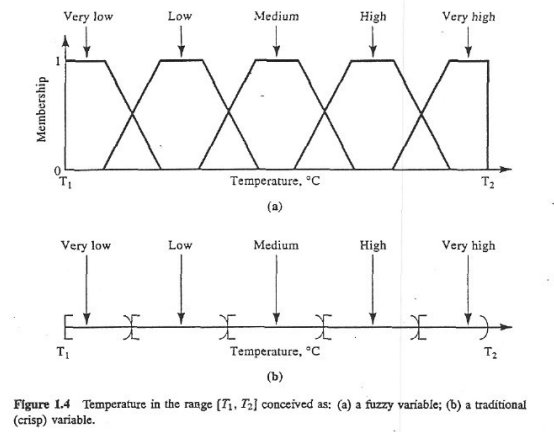
\includegraphics[scale=0.5]{Chapter1/lit-review-img/fuzzy-sets.png}
  \caption{A comparison between Fuzzy Sets and Crisp sets. \textit{Image Source: Fuzzy Sets and Fuzzy Logic: Theory and Applications \cite{GEORGE_J_BO_2008}}}
  \label{fig:fuzzy-sets}
\end{figure}

After combining Fuzzy Set Theory with Entropy, then the amount of fuzzy information gained from the fuzzy set(s) is known as fuzzy entropy.

\subsubsection{Non-Probabilistic Entropy - 1972}
\label{sssec:non-prob-review}

De Luca and Termini are considered to be the first to have taken Shannon Entropy and extended it to include fuzziness \cite{DeLuca_Termini_1972}. They also defined properties which a fuzzy entropy must follow, in order to be classed as true.

Their non-probabilistic fuzzy entropy equation is as given:

\begin{equation}\label{eq:de-luca-eq}
  H_A = -K \displaystyle\sum_{i=1}^{n}{\{\mu_i\log(\mu_i) + (1 - \mu_i)\log(1 - \mu_i)\}}
\end{equation}
\myequations{Non-Probabilistic Entropy}

Where $\mu$ is the maximum membership across all the fuzzy sets.

The entropy given by equation \eqref{eq:de-luca-eq} satisfies all 4 of De Luca and Termini's defined properties:

  \begin{subequations} \label{eq:de-luca-cond}
    \begin{align}
      &\text{\textbf{P-1 }} H_A = 0 \text{ iff } A \text{ is a crisp set (}\mu_i = 0 \text{ o r} 1 \forall x_i \in A\text{)} \\
      &\text{\textbf{P-2 }} H_A \text{ is maximum iff }\mu_i = 0.5 \forall x_i \in A \\
      &\text{\textbf{P-3 }} H \geq H^\ast\text{ where }H^\ast\text{ is the entropy of }A\text{, a sharpened version of } A \\
      &\text{\textbf{P-4 }} H = \overline{H}\text{ where }\overline{H}\text{ is the entropy of the complement set }\overline{A}
    \end{align}
  \end{subequations}


%\subsubsection{Fuzzy entropy and conditioning - 1986}

\subsubsection{Fuzzy Shannon Entropy - 1989}

Sander \cite{Sander_1989} presented a characterisation of a fuzzy entropy some time after De Luca and Termini`s work was published. His implementation of Shannon fuzzy entropy is laid out in equation \eqref{eq:fuzzy-shannon} below:

\begin{equation}\label{eq:fuzzy-shannon}
  H(f) = -c \displaystyle\sum_{i=1}^{n}{f(x_i)lnf(x_i), c > 0}
\end{equation}

Where the power of a fuzzy set is defined as:

\begin{equation}
  P(f) = \displaystyle\sum_{i=1}^{n}{f (x_i)}
\end{equation}

Sander further went on to propose some properties, which must be imposed on a fuzzy entropy $d$ to ensure that $d(f) = H(f)$:

\begin{subequations}
  \begin{align}
    &\text{\textbf{1. Sharpness: }} d(f) = 0 \Leftrightarrow f(X) \subset {0,1}, f \in [0,1]^X \\
    &\text{\textbf{2. Valuation: }} d(f \wedge g) + d(f \vee g) = d(f) + d(g), f,g \in [0,1]^X \\
    \begin{split}
    &\text{\textbf{3. Generalised additivity: }} \text{There exists two mappings s,t: } [0,\infty) \rightarrow  [0,\infty) \\
      &\text{ such that } d(f x g) = d(f)t(P(g)) + s(P(f))d(g) \text{ for all } f \in [0,1]^X, g \in [0,1]^Y, \\
      &\text{ where } X \text{ and } Y \text{ are finite sets.}
    \end{split}
  \end{align}
\end{subequations}

\subsubsection{Object-background segmentation using new definitions of entropy - 1989}

Pal \& Pal outlined their first fuzzy entropy algorithm in 1989 \cite{Pal_Pal_1989}, which satisfies all 4 of De Luca and Termini`s 4 conditions (outlined in Equations\eqref{eq:de-luca-cond}). It as as follows:

\begin{equation} \label{eq:pal-pal-orig}
  H = -k  \displaystyle\sum_{i=1}^{n}{\{\mu_iexp(1 - \mu_i) + (1 - \mu_i)exp(\mu_i)\}}
\end{equation}

\subsubsection{Higher Order Fuzzy Entropy \& Hybrid Entropy - 1992}
\label{sssec:hybrid-section}

In Pal \& Pal's paper \say{Higher order fuzzy entropy and hybrid entropy of a set} \cite{Pal_Pal_1992}, they not only prove some of De Luca \& Termini`s work to be flawed, but also defined two new fuzzy entropy algorithms, and a new set of definitions.

\noindent \textbf{Higher Order Fuzzy Entropy}

As defined by Pal \& Pal:

\begin{itemize}
  \item $P = $ Fuzzy property set
  \item $\mu =$ the degree to which $x_i$ possesses the property $P$
  \item $n =$ number of elements, with $r =$ a combination of elements from group $n$
  \item $S^r_i =$ denotes the $i$th element of such a combination
  \item $\mu(S^r_i) =$ the degree to which the combination $S'$ as a whole possesses $P$
  \item There are $\begin{bmatrix} \bigl(\begin{smallmatrix}
  n \\ r
  \end{smallmatrix} \bigr) \end{bmatrix}$ such combinations
\end{itemize}

The entropy of order $r$ of the fuzzy set $A$ is defined as:

\begin{equation} \label{eq:higher-order}
  H' = \bigg(\frac{I}{\bigl(\begin{smallmatrix}
  n \\ r
\end{smallmatrix} \bigr)}\bigg) \displaystyle\sum_{i=1}^{\bigl(\begin{smallmatrix}
  n \\ r
  \end{smallmatrix} \bigr)} \{ \mu(S^r_i)exp(1 - \mu(S^r_i)) \} + \{ 1 - \mu(S^r_i) \}log\{\mu(S^r_i)\}
\end{equation}

If $r = 1$, then \eqref{eq:higher-order} reduces to Equations \eqref{eq:pal-pal-orig} and \eqref{eq:de-luca-eq}

\noindent \textbf{Hybrid Entropy}

Another fuzzy entropy implementation outlined in Pal \& Pal`s paper was Hybrid Entropy. This algorithm is particularly useful as it combines Probabilistic and Possibilistic (fuzziness) uncertainty and if fuzziness is removed or not present, it returns to that of a classical set.

Let us define Hybrid Entropy.

\begin{itemize}
\item Let $p_0$ and $p_1$ be the probabilities of receiving 0 and 1 symbols over a noisy digital communication line respectively.
\item Let $\mu$ denote the membership functions of the fuzzy set \say{Symbol close to 1}
\item Both $E_1$ is a monotonically increasing function of $\mu$ - $E_0$ can be perceived as the likelihood (possibility) of receiving a \say{1} symbol
\begin{itemize}
    \item as $\mu$ increases from 0 to 1, then $E_1$ also increases
    \item e.g. with an incoming \say{0} symbol, if $\mu$ increases, than the difficulty of correct interpretation also \textit{increases} - a wrong interpretation of a \say{0} becomes likely
    \item e.g. for an incoming \say{1} symbol, if $\mu$ increases, then the difficulty of correct interpretation \textit{decreases} - improving likelihood of correct classification
  \end{itemize}
\item At the same time, $E_0$ can be perceived as the likelihood (possibility) of receiving the \say{0} symbol for the same reasoning
\end{itemize}

$E_0$ and $E_1$ can be defined as:

\begin{subequations} \label{eq:E0-E1}
  \begin{align}
    &E_0 = \frac{1}{n}\displaystyle\sum_{i=1}^{n}{(1-\mu_i)exp(\mu_i)} \\
    &E_1 = \frac{1}{n}\displaystyle\sum_{i=1}^{n}{\mu_iexp(1-\mu_i)}
  \end{align}
\end{subequations}

Therefore, the hybrid entropy of fuzzy set $A$ can be defined as:

\begin{equation}
  H_{hy} = -p_0\log(1 - E_0) - p_1\log(E_1)
\end{equation}

\subsubsection{Fuzzy Entropy: a Brief Survey - 2001}

Due to the older nature of some of the papers listed above, some were difficult to locate online. So when implementing the chosen algorithms (Non-Probalistic Entropy and Hybrid Entropy), Al-sharhan et al's paper \say{Fuzzy Entropy: a Brief Survey} \cite{Al-Sharhan_Karray_Gueaieb_Basir_2001} was a useful tool.

Its concise nature, and chronological listing ensured a strong understanding of the basic principles, before introducing the more complex algorithms (such as Higher Order Fuzzy Entropy). The paper also highlights advantages and flaws to each solution.

\subsection{Joint Image Alignment}

Joint image alignment, occasionally otherwise known as groupwise image alignment, focuses on the alignment of several images, into one average image. This research area has been particularly prevalent in areas such as medical and facial imagery \cite{Tiddeman_Hunter_2011} \cite{Cootes_Twining_Petrovic_Babalola_Taylor_2010}. Cootes et. al. leverage a groupwise registration algorithm to choose one base image with control points to align (typically a standard mesh frame), analyse each following image in turn estimating the movement needed to align corresponding control points, then iteratively warp each image to fit the reference frame, adjusting the texture model as they`re aligned. This type of alignment will not be considered for the project due to the over-complexity needed for the input image, along with computational limitations due to aligning one image at a time with the base image.

This Subsection will look into a couple of the techniques which will be suitable for this project.

\subsubsection{Learned-Miller`s Congealing}

Learned-Miller's \Gls{Congealing} \cite{joint-alignment} is often cited as being one of the first to truly align simple sets of data (which must have minimal noise, no occlusions and illumination variation) \cite{Zhou_Lee_Yu_Efros_2015} \cite{peng2012rasl}. Many more robust image alignment techniques have been developed off of the basis of this work, however with more computational-expense.

This algorithm works by iteratively reducing the pixel-wise entropy over the input images, using a set of standard image transformations, in a \gls{non-deterministic} manner, such as:

\begin{itemize}
  \item $x$ \& $y$ translations (Figure \ref{fig:translation})
  \item rotation (Figure \ref{fig:rotation})
  \item $x$ \& $y$ shear (Figures \ref{fig:x-shear} \& \ref{fig:y-shear} respectively)
  \item $x$ \& $y$ scale (Figure \ref{fig:scale})
\end{itemize}

\begin{center}
  \begin{figure}[H]
      \begin{subfigure}[b]{0.45\textwidth}
        \centering
            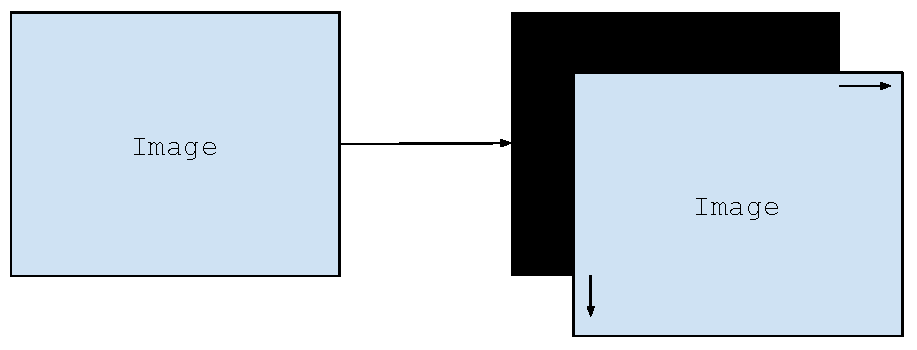
\includegraphics[width=\textwidth]{Chapter1/lit-review-img/translation.pdf}
          \caption{Image translation in the $x$ \& $y$ axes.}
          \label{fig:translation}
      \end{subfigure} \hfill
      ~ %add desired spacing between images, e. g. ~, \quad, \qquad, \hfill etc.
        %(or a blank line to force the subfigure onto a new line)
      \begin{subfigure}[b]{0.45\textwidth}
          \centering
          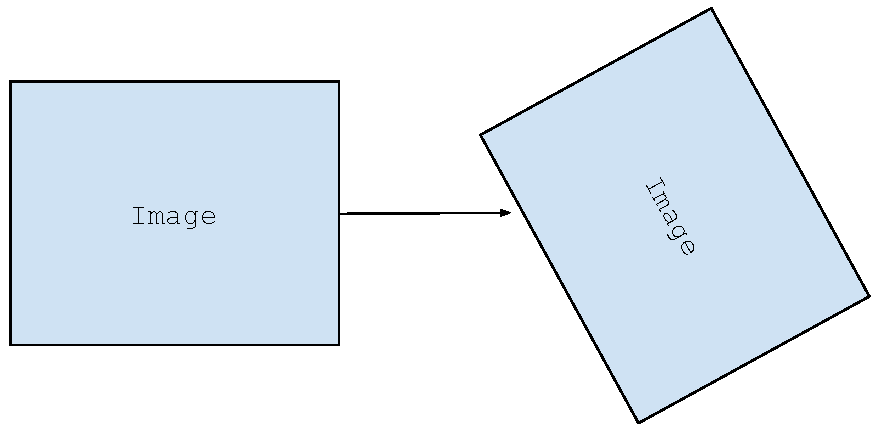
\includegraphics[width=\textwidth]{Chapter1/lit-review-img/rotation.pdf}
          \caption{Image rotation about the origin.}
          \label{fig:rotation}
      \end{subfigure}
      ~ %add desired spacing between images, e. g. ~, \quad, \qquad, \hfill etc.
      %(or a blank line to force the subfigure onto a new line)

      \begin{subfigure}[b]{0.45\textwidth}
          \centering
        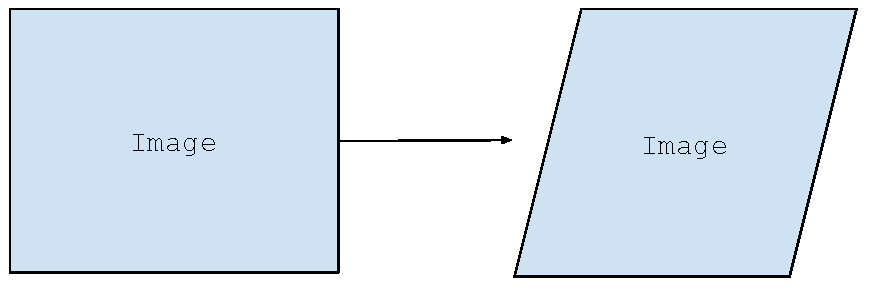
\includegraphics[width=\textwidth]{Chapter1/lit-review-img/xshear.pdf}
        \caption{Image shear in the $x$ axis.}
        \label{fig:x-shear}
      \end{subfigure} \hfill
      \begin{subfigure}[b]{0.45\textwidth}
          \centering
        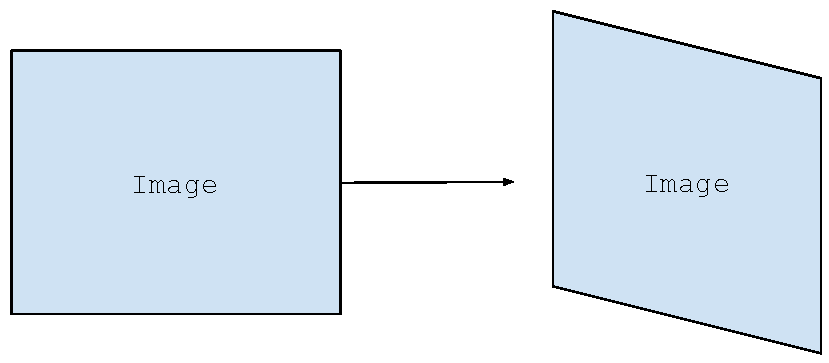
\includegraphics[width=\textwidth]{Chapter1/lit-review-img/yshear.pdf}
        \caption{Image shear in the $y$ axis.}
        \label{fig:y-shear}
      \end{subfigure}

      \begin{subfigure}[b]{\textwidth}
        \centering
        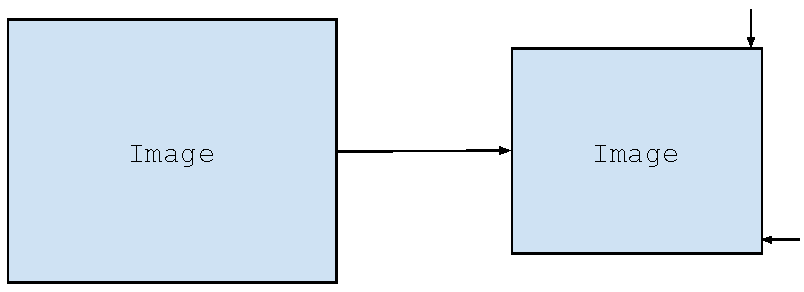
\includegraphics[width=0.45\textwidth]{Chapter1/lit-review-img/scale.pdf}
        \caption{Image scale in the $x$ \& $y$ axes.}
        \label{fig:scale}
      \end{subfigure}
    \caption{Image transformations executed by the \Gls{Congealing} algorithm}
    \label{fig:image-transformations}
  \end{figure}
\end{center}

\vspace{-1cm}

The entropy is calculated by assessing each individual set of pixel-locations in the `Pixel Stack' (see Figure \ref{fig:pixel-stack}), and by calculating the entropy of the empirical distribution of values in the Pixel Stack.

\begin{figure}[H]
  \center
  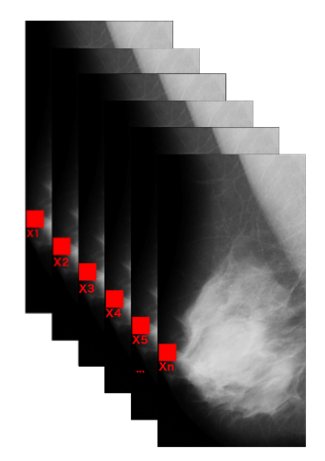
\includegraphics[scale=0.5]{Chapter1/lit-review-img/pixels.png}
  \caption{Each pixel from the same location throughout the set creates a `Pixel Stack'}
  \label{fig:pixel-stack}
\end{figure}

\subsubsection{Least squares Congealing for unsupervised alignment of images}

Further work was done upon the \Gls{Congealing} algorithm proposed by Learned-Miller by Cox et al. in 2008 \cite{Cox_Sridharan_Lucey_Cohn_2008}. They set out to address any performance issues and to remove the need for a pre-defined step size. It proposes to mitigate these issues by implementing an alternative method for aligning the images - utilising the Lucas \& Kanade algorithm for aligning a single image to another using a gradient descent approach \cite{Lucas_Kanade_1981}.

\subsubsection{Unsupervised Joint Alignment of Complex Images}

Huang and a team (notably including Learned-Miller) further extended the \Gls{Congealing} algorithm to be usable upon complex images - such as faces and cars at different orientations \cite{Huang_Jain_Learned-Miller_2007}.

This method removes the need to hand-label the input data and improves the performance of face recognition systems, by ensuring the objects are properly oriented prior to recognition.

\subsection{Image Alignment using Fuzzy Entropy}

Research has been undertaken in the past to investigate image alignment using fuzzy entropy metrics, however typically they were found to be computationally costly, and therefore slow to run on a conventional PC or laptop. This project will be investigating whether there are simpler, more light-weight fuzzy entropy metrics which could be implemented, for more everyday use in image alignment. It will also be investigated if, and further how, the outputs of these alignments differ per each fuzzy entropy metric.

Some of this work which has implemented a more computationally-costly \Gls{Congealing} algorithm is that presented by Mac Parthal\'ain and Strange in their 2013 paper \say{Fuzzy-entropy based image congealing} \cite{Mac_Parthalain_Strange_2013}.  Their implementation included dynamically-calculated fuzzy sets and a fuzzy similiarity relation matrix - allowing a comparison of all the objects to each other.

%\addcontentsline{toc}{chapter}{Development Process}
\chapter{Design}

You should concentrate on the more important aspects of the design. It is essential that an overview is presented before going into detail. As well as describing the design adopted it must also explain what other designs were considered and why they were rejected.

The design should describe what you expected to do, and might also explain areas that you had to revise after some investigation.

Typically, for an object-oriented design, the discussion will focus on the choice of objects and classes and the allocation of methods to classes. The use made of reusable components should be described and their source referenced. Particularly important decisions concerning data structures usually affect the architecture of a system and so should be described here.

How much material you include on detailed design and implementation will depend very much on the nature of the project. It should not be padded out. Think about the significant aspects of your system. For example, describe the design of the user interface if it is a critical aspect of your system, or provide detail about methods and data structures that are not trivial. Do not spend time on long lists of trivial items and repetitive descriptions. If in doubt about what is appropriate, speak to your supervisor.
 
You should also identify any support tools that you used. You should discuss your choice of implementation tools - programming language, compilers, database management system, program development environment, etc.

Some example sub-sections may be as follows, but the specific sections are for you to define. 

\section{Overall Architecture}

\section{Some detailed design}

\subsection{Even more detail}

\section{User Interface}

\section{Other relevant sections}
\subsection{Algorithm implementation}

This section will provide an outline to the implementation of the Fuzzy Entropy algorithms including the fuzzy-set membership implementation and a brief outline of the Shannon Entropy implementation provided in the demo code by Learned-Miller \cite{joint-alignment}.

More information on the new functions created, along with functions modified and utilised from the existing code base can be found in Appendix \ref{appendix:code}.

\subsubsection{Shannon Entropy}
\label{ssec:shannon-entropy}

Learned-Miller`s demo code came with an implementation of Shannon Entropy \cite{joint-alignment}. Whilst the predominant dataset was MNIST handwriting data \cite{lecun1998gradientbased}, which is a binary dataset (pixels were either black or white), this was not useful for this project as there is no variation in greyscale, even when a mean is taken of multiple images.

However, Learned-Miller had implemented code to handle the processing of greyscale and colour images, such as in MRI images. This ensured that no function needed to be created to handle grey-scale images, greatly reducing the pre-programming needed. The only image handling that was encountered was to do with the mammograms, and the creation of a large pgm file to pass into the \Gls{Congealing} algorithm, as in Section \ref{sec:tech-diff}

As outlined in \ref{ssec:entropy}, Shannon entropy is defined as:

\begin{equation}
  H(X) = - \displaystyle\sum_{i=0}^{N}{p_i \log_2 p_i}
\end{equation}

\vspace{0.5cm}
\noindent \textbf{MATLAB implementation}

This can be computed very quickly using a lookup table containing all the possible values of $p$. This makes it likely that the Shannon entropy algorithm will be the quickest on each iteration. However as it does not take any type of uncertainty into consideration when aligning the scans, the outcome could be quite dramatically different from that of a Fuzzy entropy nature.

Learned-Miller's Shannon entropy implementation has been kept, and can be found in the function \texttt{fastEntLookup.m} which is how it was originally named. Where possible, when original functions have been used, their original file names have been kept the same.

The function itself needed no changes to fit in with this project, however the way in which it is called by both \texttt{binaryCongeal.m} and \texttt{incrTrans.m} has been adapted so the user can choose which alignment metric to use when congealing their images.

\subsection{Non-Probabilistic Entropy}

\subsubsection{Fuzzy entropy description}
%==============================================================================
\label{sssec:desc}

De-Luca \& Termini fuzzy entropy algorithm \cite{DeLuca_Termini_1972} is considered to be the first to build upon Shannon entropy. Their implementation takes into account a set of data, along with their various membership degrees.


\begin{equation}
  \label{eq:de-luca}
  H_A = -K \displaystyle\sum_{i=1}^{n}{\{\mu_i\log(\mu_i) + (1 - \mu_i)\log(1 - \mu_i)\}}
\end{equation}

Al-sharhan et al's paper compiling several Fuzzy Entropy algorithms \cite{Al-Sharhan_Karray_Gueaieb_Basir_2001} contains a methodical,in-depth derivation of their algorithm, and has been instrumental in building my knowledge on the algorithm in question.

We will assume $-K$, the positive constant, is defined as $\frac{1}{n}$ as outlined in \cite{DeLuca_Termini_1972}.

%==============================================================================
\subsubsection{MATLAB implementation}
%==============================================================================

After some research into current implementations of Fuzzy Entropy algorithms in MATLAB, it was concluded the best approach would be to implement De-Luca \& Termini's algorithm from scratch. This entailed creating a membership class, which computes the grey-level membership of each pixel in the mean image (calculated from a set of input images).

This array of pixel memberships is fed into a `De Luca' function where it is iteratively passed into latter part of equation \ref{eq:de-luca} (after $\displaystyle\sum$). The output array is then summed and multiplied by $\frac{1}{n}$ as defined in Section \ref{sssec:desc}. The final mean pixel entropy is calculated by taking the image entropy and dividing by the number of pixels in the image.

This is all relatively straight forward to implement in MATLAB, as it is designed to run mathematical equations.


%==============================================================================
\subsubsection{Technical challenges}
%==============================================================================

The main technical challenge for this implementation is ensuring maximum optimisation to keep running times to a minimum. Leveraging MATLAB's own functions for the membership saves a lot of time and lines of code, however it's been important to check what they call from within. One membership function was redrawing the trapeziums every time it was called, significantly slowing down the process - reducing the amount of times the initial function was called helped reduced the run-time by over 60seconds.

Another technical challenge faced whilst implementing the De Luca \& Termini algorithm, isn't directly tied to the implementation of their specific equation, but more of my lack of experience in MATLAB, slowing down the programming rate. It has indeed been a steep learning curve, getting to grips with standard error messages, the debugger tool and knowing which `Toolboxes' are needed to run specific MATLAB functions.

Finally, as can be ascertained from Figure \ref{fig:mammo-results}, when writing the 4 seperate scans into 1 larger file, somewhere the images get rotated. This will be a reoccurring issue through the 3 Fuzzy entropy implementations, however as this is the first I will note it here. I think this is caused thanks to the swapping of the height and width values, however upon initial inspection of the file writing function, it is not clear as to which line is causing this issue. This issue has been marked low priority in the short term, due to all the scans being rotated in this fashion, and as such all have the same orientation. This means the congealing algorithm can work with no issues upon these images, the rotation is more merely an aesthetic issue.

%==============================================================================
\subsubsection{Results}
%==============================================================================

\begin{figure}[!ht]
  \centering
  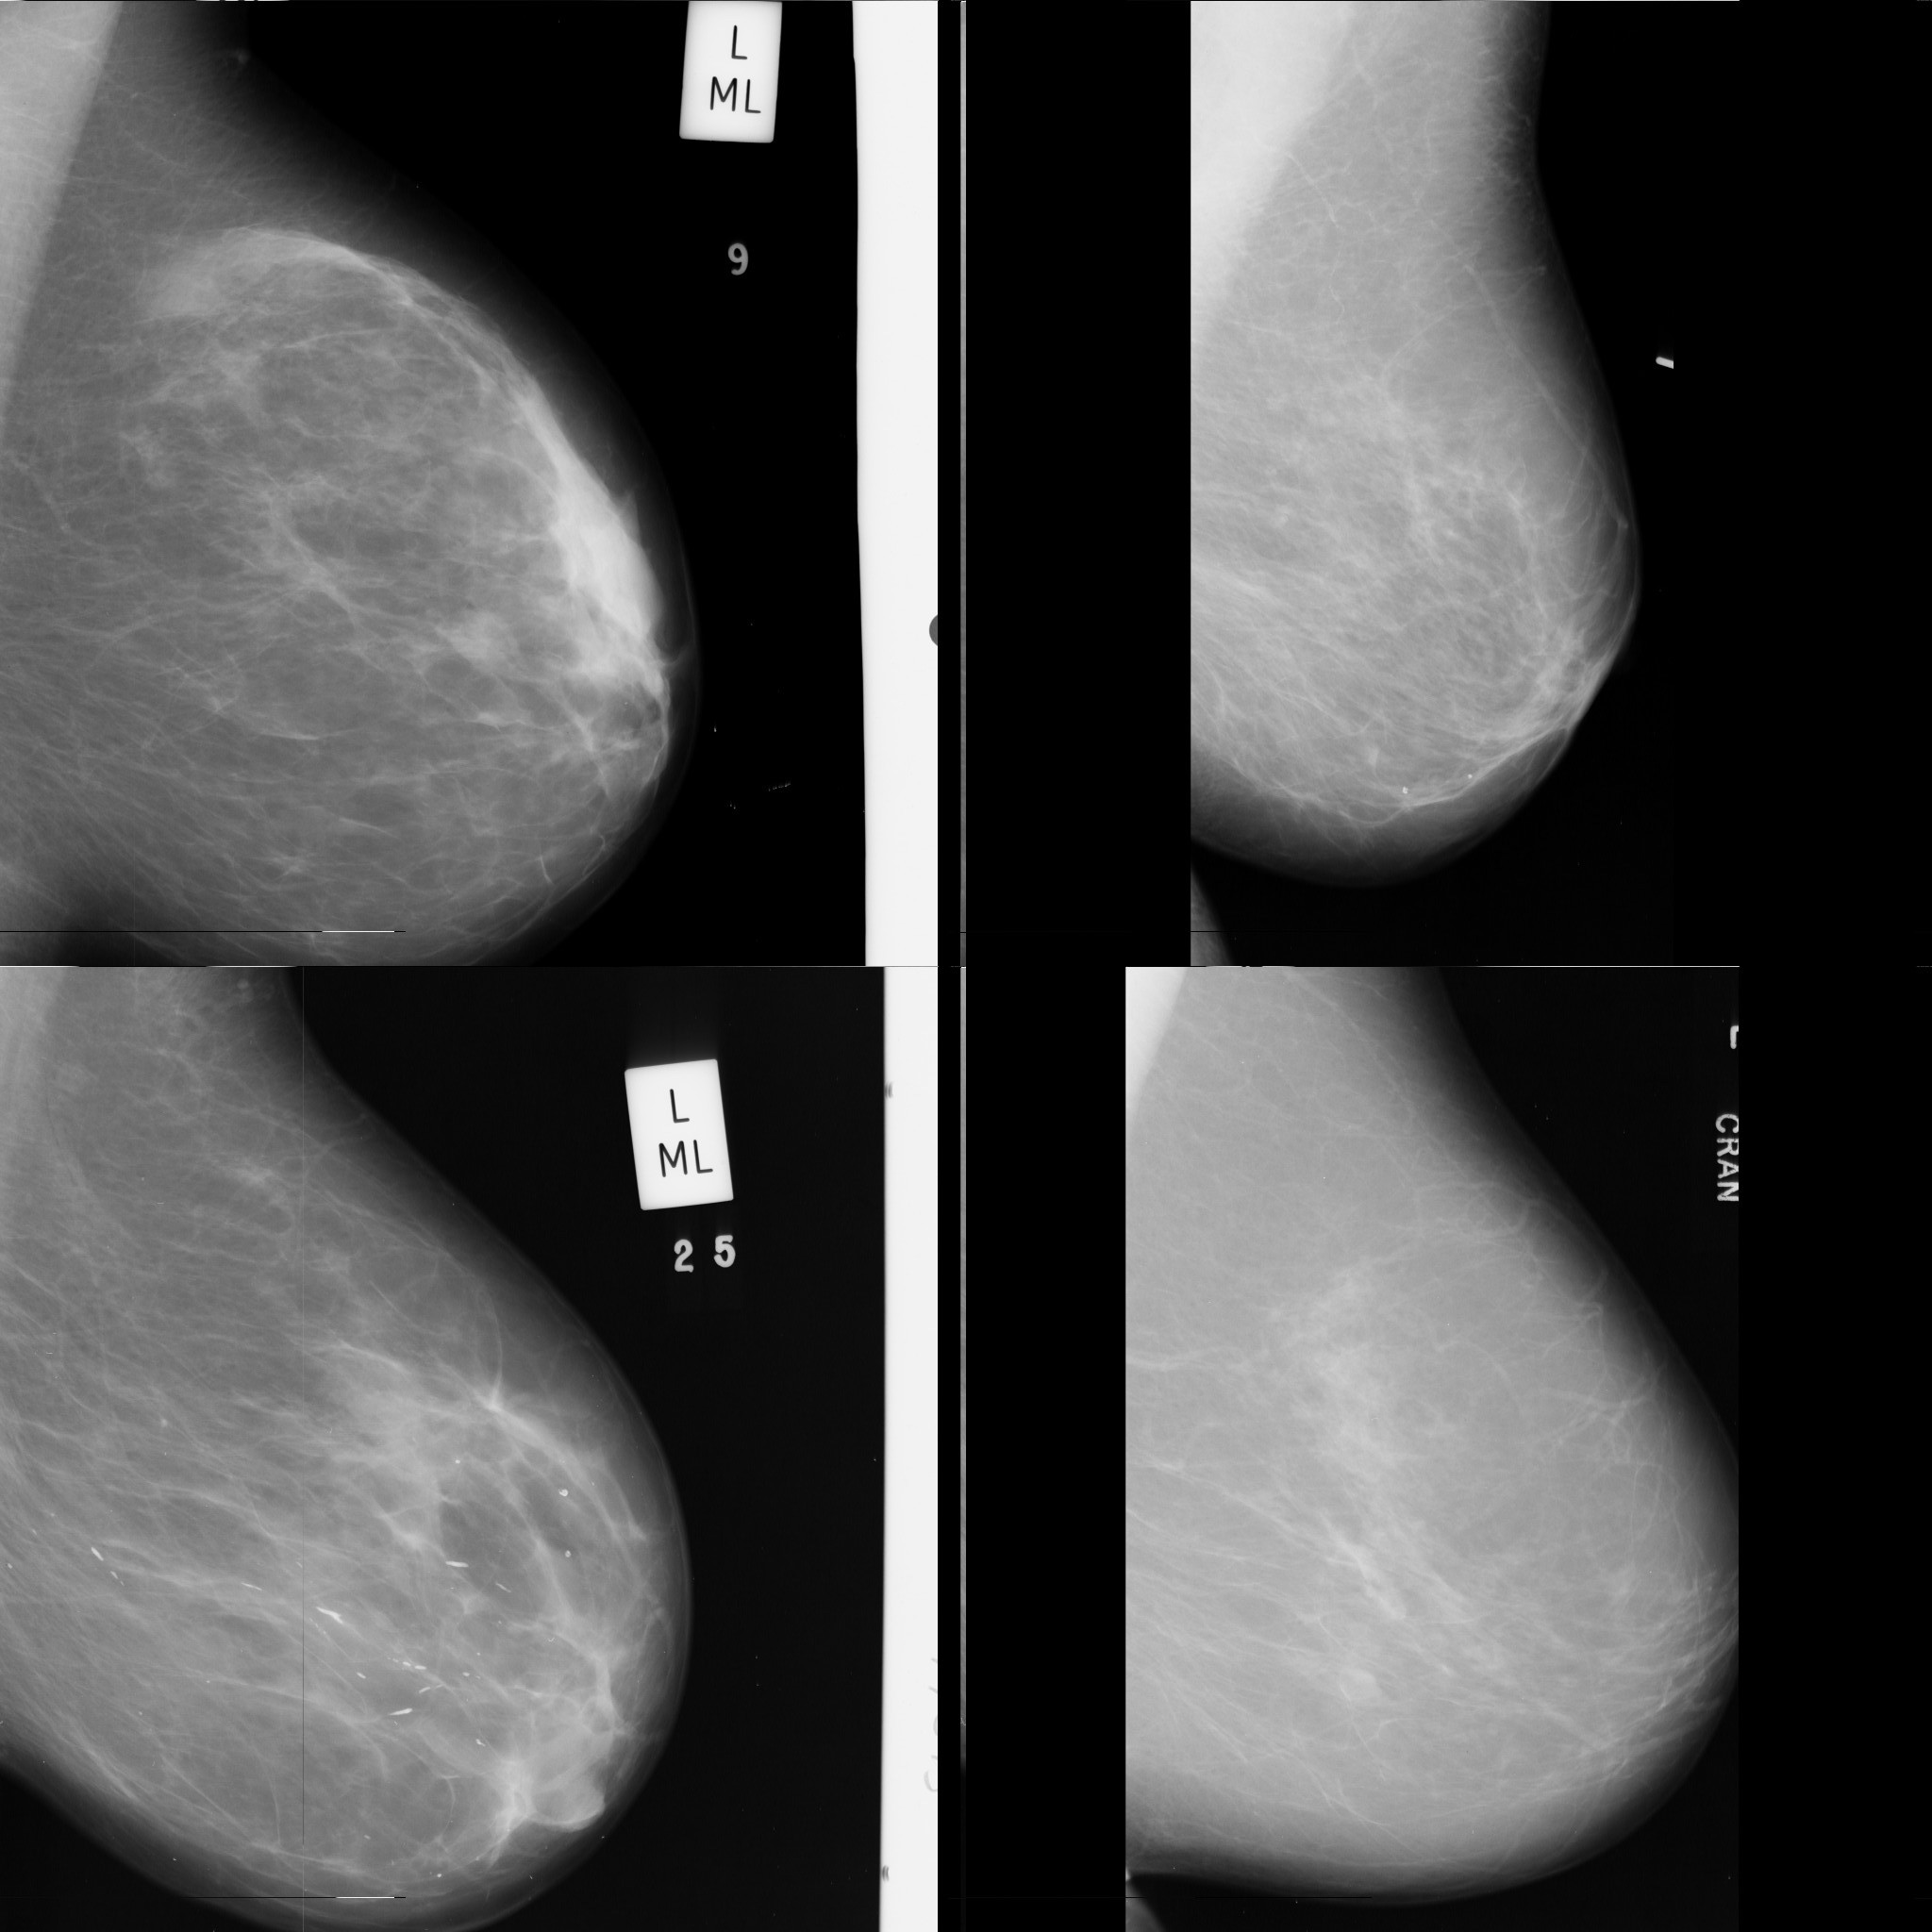
\includegraphics[width=0.4\textwidth]{Chapter2/non-prob-img/big_scan_1.jpg}
  \caption{4 input images of BI-RADS I classification}
  \label{fig:input}
\end{figure}

\begin{figure}[!ht]
    \centering
    \begin{subfigure}[b]{0.4\textwidth}
        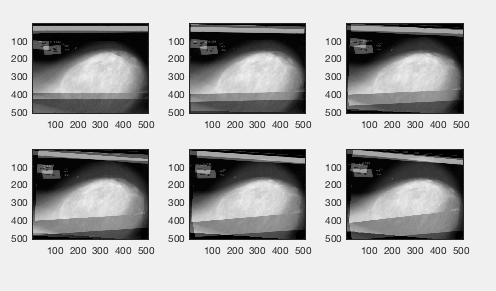
\includegraphics[width=\textwidth]{Chapter2/non-prob-img/iteration-mean.png}
        \caption{Mean image over each iteration}
        \label{fig:mean-imgs}
    \end{subfigure}
    ~ %add desired spacing between images, e. g. ~, \quad, \qquad, \hfill etc.
      %(or a blank line to force the subfigure onto a new line)
    \begin{subfigure}[b]{0.4\textwidth}
        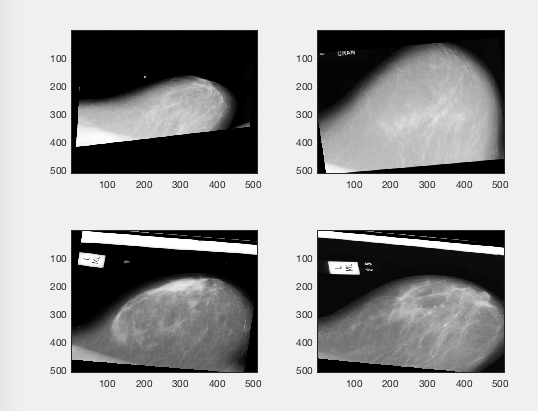
\includegraphics[width=\textwidth]{Chapter2/non-prob-img/adj-ser.png}
        \caption{Adjusted original input images}
        \label{fig:adj-ser}
    \end{subfigure}
    \caption{Output of 5 congealing iterations}\label{fig:mammo-results}
\end{figure}

\begin{figure}[!ht]
  \centering
  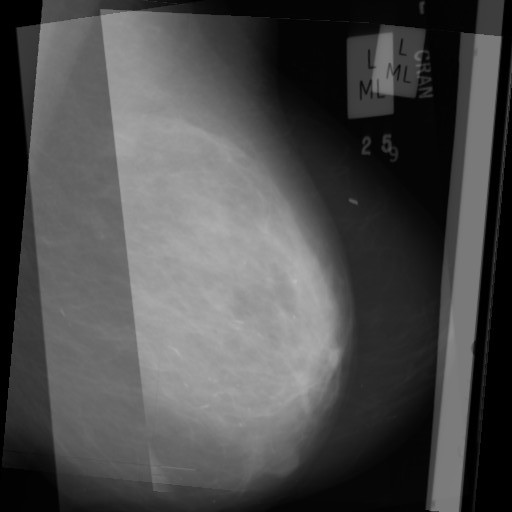
\includegraphics[width=0.4\textwidth]{Chapter2/non-prob-img/final_mean.jpg}
  \caption{Final mean image after 5 iterations (bottom-right most in Figure \ref{fig:mammo-results})}
  \label{fig:final-mean}
\end{figure}

\subsubsection{Entropy results}

  \begin{tabular}{ | l | r | }
    \hline
    \textbf{Iteration} & \textbf{Entropy} \\
    \hline
    1 & 0.050519 \\ \hline
    2 & 0.043925 \\ \hline
    3 & 0.035679 \\ \hline
    4 & 0.029035 \\ \hline
    5 & 0.026194 \\ \hline
  \end{tabular}

\subsubsection{Time to Run}

\begin{figure}[!ht]
  \centering
  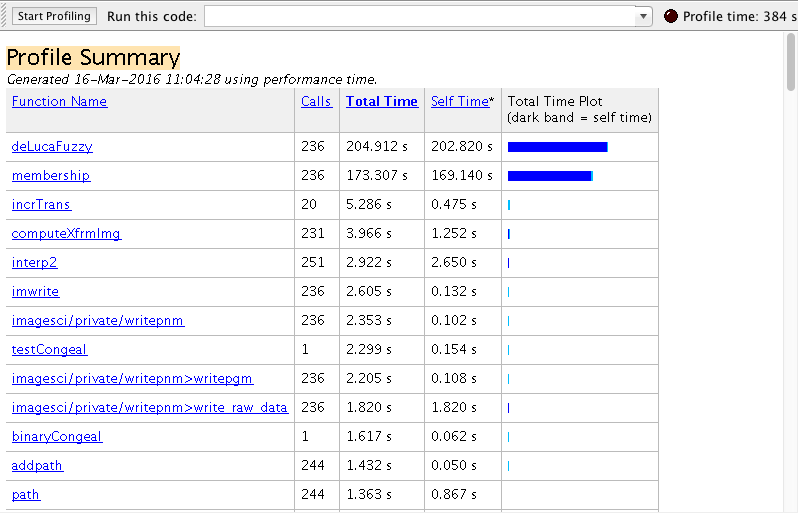
\includegraphics[width=0.8\textwidth]{Chapter2/non-prob-img/Run-time.png}
  \caption{Snapshot of run-time statistics}
  \label{fig:run-time}
\end{figure}

\subsection{Hybrid Entropy}

As mentioned in Section \ref{sssec:hybrid-section}, the Hybrid Entropy equation is as follows:

\begin{equation}
  H_{hy} = -p_0\log(1 - E_0) - p_1\log(E_1)
\end{equation}

Where $E_0$ and $E_1$ can be defined as:

\begin{subequations} \label{eq:E0-E1}
  \begin{align}
    &E_0 = \frac{1}{n}\displaystyle\sum_{i=1}^{n}{(1-\mu_i)exp(\mu_i)} \\
    &E_1 = \frac{1}{n}\displaystyle\sum_{i=1}^{n}{\mu_iexp(1-\mu_i)}
  \end{align}
\end{subequations}

And $p_0$ and $p_1$ are the probabilities of receiving 0 and 1 symbols respectively.

%==============================================================================
\subsubsection{MATLAB implementation}
%==============================================================================

Due to reasons covered in the Subsubsection \ref{sssec:hyrid-technical}, Hybrid Entropy membership was implemented using 2 trapeziums covering 2 fuzzy sets, as seen in Figure

\begin{figure}[H]
  \center
  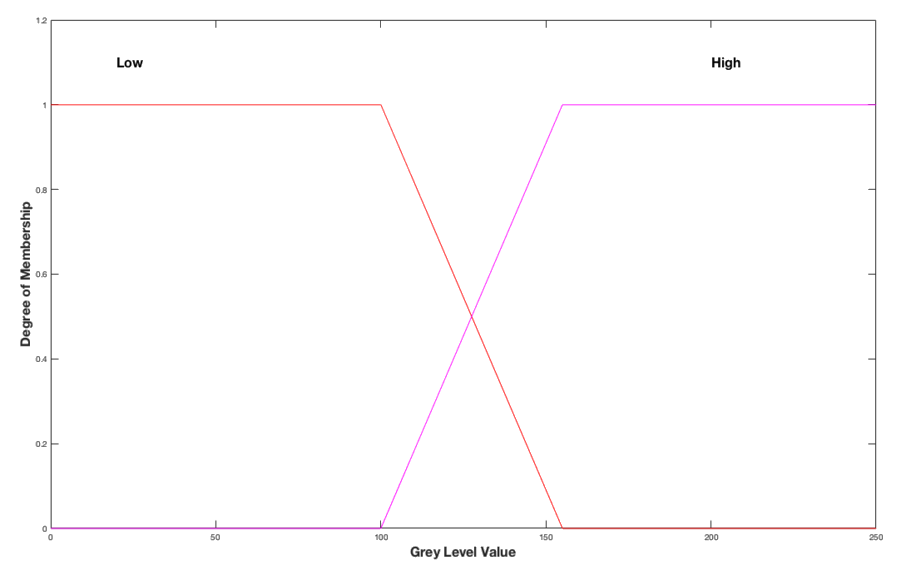
\includegraphics[scale=0.5]{Chapter2/hybrid-img/2_traps.png}
  \caption{Two membership trapeziums for Hybrid Entropy - Low and High grey-level values.}
  \label{fig:2-traps}
\end{figure}

Two arrays are then fed into the Hybrid Entropy function - one listing all the pixel membership values from the low trapezium, and the other from the high trapezium. The final entropy is taken as a comparison between the low and high fuzzy sets.

%==============================================================================
\subsubsection{Technical challenges}
\label{sssec:hyrid-technical}
%==============================================================================

Whilst Hybrid Entropy utilises a membership function, much like Non-Probabilistic entropy, it was derived to work with binary entropy, not the ternary membership modeled for Non-Probabilistic. Because of the binary nature, the equation uses `inversion' to depict if not this fuzzy set, then must belong to the other.

Experimentation was done as to whether the equation could be adapted in such a way to continue using three separate membership trapeziums - low, medium and high grey-level values.

\textbf{Initial ideas - check email between me and neil}


Logic would dictate that if the comparison of two fuzzy sets works, then to compare the low fuzzy set to the medium, the medium to the high and the high to the medium should work.

For example:

\begin{figure}[!ht]
  \centering
  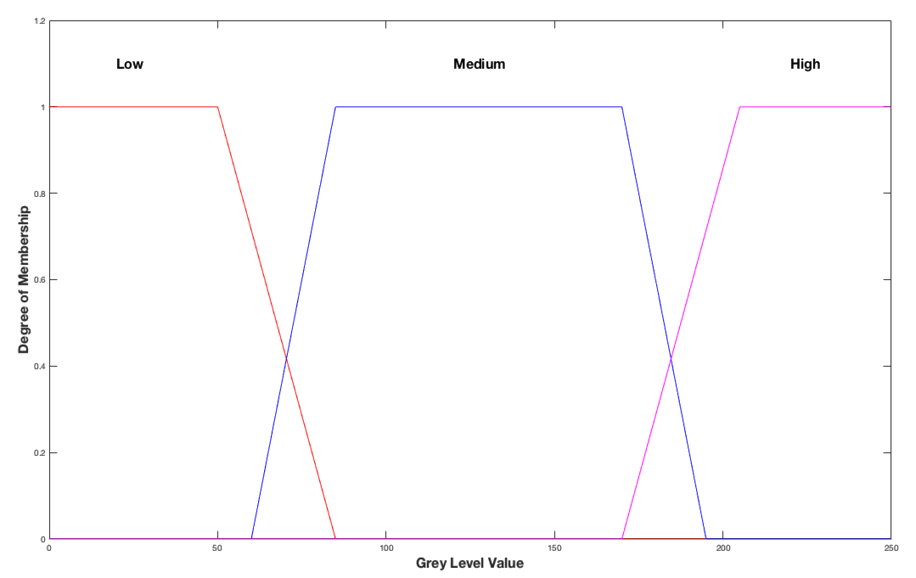
\includegraphics[scale=0.5]{Chapter2/hybrid-img/3_traps.png}
  \caption{3 fuzzy set trapeziums}
  \label{fig:3-traps}
\end{figure}

In theory, calculating $E_0$ and $E_1$ for each trapezium, calculating the hybrid entropy for each, and then combining them, should work:

\begin{equation}
E_0 = \frac{1}{No.\_of\_pixels\_in\_low\_trapezium}\displaystyle\sum_{i=1}^{n}{(1-Low\mu_i)exp(Low\mu_i)}
\end{equation}
\begin{equation}
E_1 = \frac{1}{No.\_of\_pixels\_in\_low\_trapezium}\displaystyle\sum_{i=1}^{n}{Low\mu_iexp(1-Low\mu_i)}
\end{equation}

Where $Low\mu$ is the membership of the pixels in the low fuzzy set.
%http://tex.stackexchange.com/questions/112238/how-to-wrap-a-long-equation-in-latex
\begin{equation}
H_{hy} = -p_0\log_{10}(1 - E_0) - p_1\log_{10}(E_1)
\end{equation}

Where

$p_0 = \frac{No.\_of\_pixels\_in\_low\_trapezium}{No.\_of\_pixels\_in\_low\_trapezium + med\_trapezium}$

and

$p_1 = \frac{No.\_of\_pixels\_in\_med\_trapezium}{No.\_of\_pixels\_in\_low\_trapezium + med\_trapezium}$


This was done for all 3 trapeziums, then combined and divided by 3 (for the mean entropy). As the result for each trapezium should be between 0 and 1 (as each is an entropy value), then combining them should be no issue. However this was not the case.

First of all, the hybrid equation output was deemed to be `NaN' - something which generally occurs when attempting to divide by 0. Anomalous outputs from the high trapezium was to be expected, as there are very few pixels which fall within the range nearer the white end of the grey-level scale. This was mitigated by setting the output equal to 0, in effect ignoring any output from the highest fuzzy set.

After this mitigation, the third and fourth iteration had suitable entropy values, however the fifth entropy value was a negative, something which is not possible in terms of entropy, as it must be between 0 and 1 - see Figure \ref{fig:minus-entropy}.

\begin{figure}[H]
  \begin{center}
  %  \pgfplotsset{every axis/.append style={thick},width=0.4*\textwidth, ymax=1}
  %    \begin{tikzpicture}
  %        width = 10cm,
  %        axis lines = middle,
  %        xlabel = {Iterations},
  %        ylabel = {Entropy},
  %        ymin = -0.3,
  %        ymax = 0.3,
  %        ytick={-0.5,-0.4,...,0.6},
  %        y tick label style={
  %                /pgf/number format/.cd,
  %                fixed,
  %                fixed zerofill,
  %                precision=1,
  %            /tikz/.cd
  %        },
  %        xtick={1,2,...,5},
  %        x label style={at={(axis description cs:0.5,0.3)},anchor=north},
  %        y label style={at={(axis description cs:-0.1,.5)},rotate=90,anchor=south},
  %        nodes near coords,
  %    	  nodes near coords align={vertical},
  %        every node near coord/.append style={font=\scriptsize,
  %                xshift = +3pt, yshift=+4pt,anchor=west, /pgf/number format/precision=6},
  %        ]
  %      \addplot coordinates
  %        { (1, 0.124512) (2, 0.048099) (3, 0.238875) (4, 0.232505) (5, -0.140011) };
  %        \draw[ultra thin] (axis cs:0,\pgfkeysvalueof{/pgfplots/ymin}) -- (axis cs:0,\pgfkeysvalueof{/pgfplots/ymax});
  %      \end{axis}
  %    \end{tikzpicture}
    \end{center}
    \caption{Graph showing the entropy output after 5 iterations}
    \label{fig:minus-entropy}
\end{figure}

It was concluded that the implementation of three fuzzy sets within Hybrid Entropy would not be realistic within the remaining timeframe of the project, and the membership for Hybrid Entropy was redefined to the concept of 2 fuzzy sets, as set out by Pal and Pal. This would mean, one trapezium for pixel grey-level values with low values, overlapping with a high grey-level value trapezium at approximately 128, as seen in Figure \ref{fig:2-traps}.

%==============================================================================
\subsubsection{Run-time}
%==============================================================================

\section{Software}

\subsection{Methodology}

In the past, software projects followed a strict-plan driven approach, such as the Waterfall method, however more recently, Agile practices have become widely accepted, allowing the developer more freedom. This features an iterative development approach, with short \say{iterations} or \say{sprints} defined in which the developer should complete a block of work, typically a \say{story} or \say{feature} given the Agile methodology chosen.

The Agile Methodology has a manifesto \cite{Manifesto}, which perfectly encompasses all the values it strives to achieve:
\begin{itemize}
  \item \textbf{Individuals and interactions} over processes and tools
  \item \textbf{Working software} over comprehensive documentation
  \item \textbf{Customer collaboration} over contract negotiation
  \item \textbf{Responding to change} over following a plan
\end{itemize}

\begin{quotation}
  \textit{That is, while there is value in the items on the right, we value the items on the left more.}
\end{quotation}

Scrum is one of the most popular interpretations of an Agile Methodology, due to it's simplicity \cite{scrum}. Scrum is \textit{not} an agile methodology, however is a framework, to which agile practices such as Pair Programming and \acrfull{TDD} can be aligned.

Given it's flexible and light-weight nature, an adapted Scrum methodology has been undertaken for this project. The flexible nature is particularly useful given the research nature of this project, as the requirements were not fully defined at the start of the process, and changed as time went on given the outcome of experimentation with mathematical concepts for image alignment.

Additionally, \acrfull{XP} \cite{xp} dates back to 1996, and is one of the most recognisable Agile Methodologies used in the software industry currently. \acrshort{XP} claims to create successful software projects by following 5 key principles:

\begin{itemize}
  \item \textbf{Communication: } constantly communicate with their customers and fellow programmers
  \item \textbf{Simplicity:} keep the design simple and clean
  \item \textbf{Feedback:} testing the software starting on day one
  \item \textbf{Respect: } every small success deepens their respect for the unique contributions of each and every team member
  \item \textbf{Courage: } deliver the system to the customers as early as possible and implement changes as suggested
\end{itemize}

Given that this project is a single-person project, neither framework/methodology would work well on it's own, so for this project, it was decided that Scrum would be the main framework, with elements of XP to help strengthen areas such as design and testing.

\subsubsection{Tools to manage methodology}

This project has been chiefly supported by the tool \url{taiga.io} - a beta web app \cite{Taiga.io}, which aims to promote the use of Scrum and Kanban \cite{kanban}.

Having an online app to organise User Stories, Tasks, Issues and to track progress using a Burndown chart was extremely important in this single-person project, where work was carried out across several different devices and platforms. It also ensures a historical record of what was completed, and when, as is evident from Subsubsection \ref{sssec:user-stories}.

\subsubsection{User stories}
\label{sssec:user-stories}

User Stories are a bid to shift away from talking in technical-jargon, and to shift towards talking in plain english about project requirements. When working with a customer, this is obviously useful, as occasionally they can be non-technical, so this helps promote an open-dialogue between customer and developer, and a clear understanding of the customer's needs.

User Stories typically follow a template for consistency, usually something similar to:

\begin{quotation}
  \textit{As a $<$type of user$>$, I want $<$some goal$>$ so that $<$some reason$>$.} \cite{user_story}
\end{quotation}

User Stories also have associated Story Points, which is a typically a numbering system leveraged to indicate the effort needed to implement the Story. Due to the uncertain nature of programming, it is not always an accurate reflection of effort, however through the Agile community it is generally accepted that to be consistent in your assignment of points is more useful than being accurate \cite{estimation}. During the early stages of the project, it is often the case in which estimation is a little off what it should be, however as the project progresses, and the developer gains a better understanding of the tasks, and how to implement them, then estimation tends to become more accurate.

Table \ref{table:User Stories} outlines the User Stories used during this project, along with when they were working upon (during which Sprint) and how many Story Points are associated with it.

\begin{center}
  \small
  \begin{longtable}{| p{2cm} | p{4cm} | p{2cm}  | p{2cm} | p{3cm} |}
    \hline
      \textbf{Reference} & \textbf{User Story} & \textbf{Milestone} & \textbf{Story Points} & \textbf{Additional Comments} \\ \hline \endhead
      1 & Clinicians can upload a set of images (MATLAB Command Window) so they can control what images are input into the \Gls{Congealing} Algorithm & Sprint 0 & 5 & \\ \hline
      2 & Developer will implement membership of a pixel so that Fuzzy Entropy can be calculated & Sprint 1 & 10 & \\ \hline
      3 & Clinicians can align scans using Non-Probabilistic Entropy so it can be used in the \Gls{Congealing} Algorithm & Sprint 2 \& 3 & 20 & Due to complexity of the implementation, this was spread over 2 sprints \\ \hline
      4 & Clinicians can select an alignment metric (MATLAB Command Window) so they can select which to align the images using & Sprint 4 & 5 & \\ \hline
      5 & Developer will make standard GUI with no functionality so that this can be demoed as a proof of concept & Sprint 4 & 5 & \\ \hline
      6 & Clinician can choose number of iterations (MATLAB Command Window) so they can run as many as they want to & Sprint 4 & 3 & \\ \hline
      7 & Developer will implement Basic mammogram upload so that they can be aligned & Sprint 4 & 8 & \\ \hline
      8 & Clinicians can align scans using standard Entropy so it can be used in the \Gls{Congealing} Algorithm & Sprint 5 & 8 & \\ \hline
      9 & Clinicians can upload a set of images - GUI & Sprint 5 & 10 & \\ \hline
      10 & Developer will optimise membership function so as to improve performance & Sprint 5 & 2 & Promoted from an Issue \\ \hline
      11 & Developer will optimise Non-Probabilistic Function so as to improve performance & Sprint 5 & 2 & Promoted from an Issue \\ \hline
      12 & Clinicians can clear an input image so that they can reselect an input image & Sprint 5 & 3 & \\ \hline
      13 & Clinicians can align scans using Hybrid Entropy so it can be used in the \Gls{Congealing} Algorithm  & Sprint 6 & 20 & \\ \hline
      14 & Clinicians can select an alignment metric from a drop-down menu so it is easy to choose which alignment metric to use & Sprint 6 & 5 & \\ \hline
      15 & Clinicians can select the number of iterations to be run using an alignment metric (GUI) so it is easy to select how many iterations to run & Sprint 6 & 5 & \\ \hline
      16 & Clinicians can see meta data about the input image so they can see if the uploaded image is the correct one & Sprint 6 & 2 & \\ \hline
      17 & Clinicians can see each iteration mean image so they can compare the improvement over each iteration & Sprint 6 & 3 & \\ \hline
      18 & Clinicians can see adjusted input images on final iteration so they can see how the input images have changed by the final iteration & Sprint 6 & 3 & \\ \hline
      19 & Developer wants to know why Scans are rotated 90 to left as this is aesthetically displeasing & Sprint 7 & 8 & Promoted from an Issue \\ \hline
      20 & Developer will research and implement removal of Medical Markers as this causes alignment issues & Sprint 7 & 5 & \\ \hline
      21 & Clinicians can discard (clear) an alignment so they can start a new alignment & Sprint 8 & 5 & \\ \hline
      22 & Clinicians can click on average image to view it bigger so they can see the detail easier & Sprint 8 & 2 & \\ \hline
      23 & Clinicians can save the final mean image with a sensible name so they can easily find it again & Sprint 8 & 3 & \\ \hline
      24 & Clinicians can see the iteration details so they can understand more about the improvement & Sprint 8 & 8 & \\ \hline
      25 & Clinicians can see \Gls{Congealing} is running so they know it's in progress & Sprint 8 & 3 & \\ \hline
  \caption{User stories defined during the project}
  \label{table:User Stories}
\end{longtable}
\end{center}

\subsubsection{Burndown chart}

\begin{figure}[H]
  \centering
  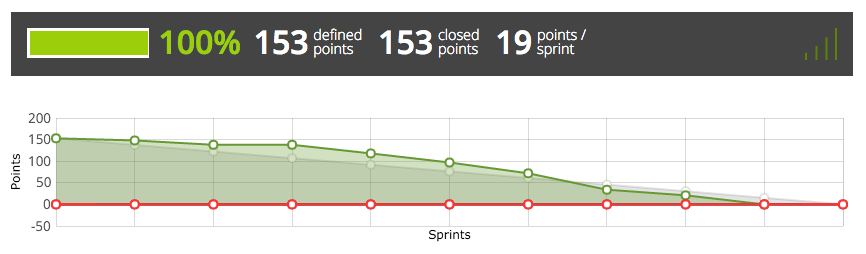
\includegraphics[width=\textwidth]{Chapter2/software-img/burndown.png}
  \caption{Project Burndown chart.}
  \label{fig:burndown}
\end{figure}

Figure \ref{fig:burndown} is a graphical representation of progress per week, as utilised in Scrum, called a Burndown chart. It allows the developer(s) a quick reference as to the progress of the project, and works by subtracting completed Story points as they're completed. Taiga includes the trend line which sets a target for completion per Sprint.

In Taiga, it was also possible to have a weekly burndown chart, so as to track progress throughout the week, rather than just the entire project.

\subsubsection{Sprint Review \& Retrospective}

Sprint Reviews are held at the end of each Sprint, to assess what work was done during the week, and does the end product match the Sprint Goal set out at the start of the week. In this project, Sprint Goals and Sprint Reviews took shape in the form of an informal online blog. Sprints were defined as a week long in this project, running between supervisor meetings (Monday - Sunday). Weekly posts would outline what had been completed that week, how things went (good and bad) and what was to be completed during the following week. Whilst less structured than the conventional approach to Reviews, it works well within a single-person project, and was a good reflection of what had been accomplished.

In Agile Methodologies, Retrospectives are typically at the end of each Sprint, so the team can assess:
\begin{itemize}
  \item What works well
  \item What doesn't work well
  \item What should they start doing
\end{itemize}

\subsubsection{Daily Standup}

Daily standups are a vital part of Scrum`s teamwork ethos. Each morning (or during a set allotted time), the time would meet to discuss what was accomplished the day before, what are the plans for the day ahead, and what road-blocks are in their way. This provides the developer (and further the team) a clear picture of what has yet to be done, and allows fellow team-mates to offer expertise to help overcome obstacles. Whilst this project is not being developed by a team, the benefit of daily standups to productivity, organisation and planning still stands, along with the crowd-sourcing element of expertise.

Throughout the project, stand ups have been held with peers, who're also working upon their Major Projects. Whilst not daily, they tended to fall bi-daily, and it gave the developer a chance to hone skills in explaining the project to people not well-versed in the subject. It was also a good breeding ground for new ideas, and an open forum for discussion into the pros and cons of certain approaches.

\subsection{Design}

In traditional plan-driven methodologies, such as the Waterfall method, Design would take shape in the form of a Design document where all the requirements would be outlined and written up in detail. As mentioned previously, this would be impractical for such a fluid, experimental project, so practices were leveraged from \acrfull{XP} to ensure that the system design was not compromised by the lack of early, solid requirements.

\subsubsection{CRC Cards}

In \acrshort{XP}, \acrfull{CRC} Cards are an useful task in which the entire team can collaborate in the system design. Whilst there is no team in this project, they still play a vital role in structuring the system, can be iteratively updated and are easily discardable should the need arise.

Typically \acrshort{CRC} cards would represent Objects, with the class of the written at the top, the responsibilities down the left and the collaborating classes down the right-hand side. However as mentioned in Section \ref{ssec:matlab}, MATLAB is built around a scripting language, and all the \say{Classes} in this project are replaced by Functions and Scripts. Therefore, each \acrshort{CRC} card represents a function or a script, and it's corresponding responsibilities and collaborations as normal - see Figure \ref{fig:crc} and Appendix \ref{appendix:crc-cards} for more detail.

\begin{figure}[H]
  \center
  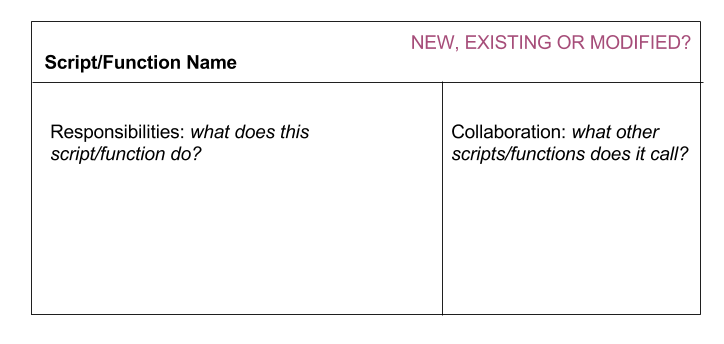
\includegraphics[scale=0.5]{Chapter2/software-img/crc.png}
  \caption{Example CRC Card as used in this project}
  \label{fig:crc}
\end{figure}

\subsubsection{GUI Design}

The name \say{Enantiomorph} was chosen as the application name as a more concise, recognisable alternative to the project title.

\begin{quotation}
  \textit{either of a pair of crystals (as of quartz) that are structural mirror images \ref{enantiomorph}}
\end{quotation}

This section will look at the design evolution of the application GUI.

\begin{figure}[H]
  \center
  \includegraphics[scale=0.5]{Chapter2/software-img/wireframe_1.png}
  \caption{Initial wireframe design for GUI}
  \label{fig:wireframe1}
\end{figure}

The initial design, as represented in Figure \ref{fig:wireframe1}, was designed to incorporate the first set of project requirements.

\begin{figure}[H]
  \center
  \includegraphics[scale=0.5]{Chapter2/software-img/wireframe_2.png}
  \caption{Second wireframe design for GUI}
  \label{fig:wireframe2}
\end{figure}

Figure \ref{fig:wireframe2} represents the changes in requirements as the project progressed. It became clear that a load button which allowed the user to \textit{both} generate a large pgm file from a folder of mammograms, or upload a large pgm file that already exists would be difficult to implement. Therefore the button got split into two, with appropriate text above the buttons to help the user decide which to use.

By the second \acrshort{GUI} iteration, it became apparent that implementing a way in which to stop the \Gls{Congealing} algorithm automatically would be too time-consuming for the time left in the project. Therefore the user would have to specify how many iterations they would like to run. This meant a textbox with numerical validation had to be incorporated into the \acrshort{GUI} and the extra iteration information fed into the back-end.

During the second application iteration, the outputs of each iteration mean and the adjusted input images were implemented for the user to see.

\begin{figure}[H]
  \center
  \includegraphics[scale=0.5]{Chapter2/software-img/wireframe_3.png}
  \caption{Third wireframe design for GUI}
  \label{fig:wireframe3}
\end{figure}

The final wireframe created is outlined in Figure \ref{fig:wireframe3}. Additional information  about the \Gls{Congealing} process can be accessed via the button in the bottom left corner and meta data about the input image displayed in the top section. Users can also clear the entire \acrshort{GUI} to start a new alignment - this could be useful should they wish to compare the outputs from the 3 different entropy alignment techniques.

\vspace{3cm}
\noindent \textbf{The final \acrshort{GUI}}

\begin{figure}[H]
  \center
  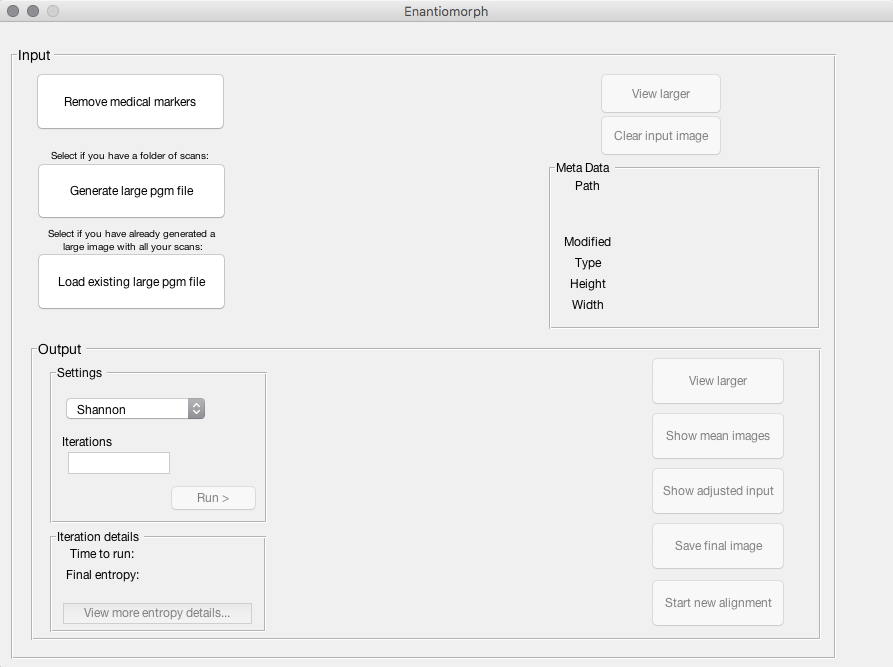
\includegraphics[scale=0.5]{Chapter2/software-img/final_gui.png}
  \caption{Final GUI}
  \label{fig:final_gui}
\end{figure}

Figure \ref{fig:final_gui} is a screenshot of the final application the user would use. This provides a more detailed insight into the finer details of the \acrshort{GUI}, more so than the previous wireframes.

\chapter{Results and Conclusions}

%This section should discuss issues you encountered as you tried to implement your experiments. What were the results of running the experiments? What conclusions can you draw from these results?

%During the work, you might have found that elements of your experiments were unnecessary or overly complex; perhaps third party libraries were available that simplified some of the functions that you intended to implement. If things were easier in some areas, then how did you adapt your project to take account of your findings?

%It is more likely that things were more complex than you first thought. In particular, were there any problems or difficulties that you found during implementation that you had to address? Did such problems simply delay you or were they more significant?

%If you had multiple experiments to run, it may be sensible to discuss each experiment in separate sections. 

\chapter{Critical Evaluation}

Examiners expect to find in your dissertation a section addressing such questions as:

\begin{itemize}
   \item Were the requirements correctly identified? 
   \item Were the design decisions correct?
   \item Could a more suitable set of tools have been chosen?
   \item How well did the software meet the needs of those who were expecting to use it?
   \item How well were any other project aims achieved?
   \item If you were starting again, what would you do differently?
\end{itemize}

Such material is regarded as an important part of the dissertation; it should demonstrate that you are capable not only of carrying out a piece of work but also of thinking critically about how you did it and how you might have done it better. This is seen as an important part of an honours degree. 

There will be good things and room for improvement with any project. As you write this section, identify and discuss the parts of the work that went well and also consider ways in which the work could be improved. 

Review the discussion on the Evaluation section from the lectures. A recording is available on Blackboard. 

% add any additional chapters here

\setemptyheader
\addcontentsline{toc}{chapter}{Appendices}
\chapter*{Appendices}
\pagebreak

% start the appendix - sets up different numbering
\fancypagestyle{plain}{%
%\fancyhf{} % clear all header and footer fields
\fancyhead[L]{\textsl{Appendix\ \thechapter}}
\fancyhead[R]{\textsl{\leftmark}}}

\appendix
\fancyhead[L]{\textsl{Appendix\ \thechapter}}
\fancyhead[R]{\textsl{\leftmark}}
\fancyhead[C]{}
\fancyfoot[C]{\thepage}
\renewcommand{\headrulewidth}{0.4pt}
\renewcommand{\chaptermark}[1]{\markboth{#1}{}}

\fancyhead[L]{\textsl{Appendix\ \thechapter}}
\fancyhead[R]{\textsl{\leftmark}}
\fancyfoot[C]{{\thepage} of \pageref{LastPage}}

% include any appendices here
\chapter{Third-Party Code and Libraries}

If you have made use of any third party code or software libraries, i.e. any code that you have not designed and written yourself, then you must include this appendix. 

As has been said in lectures, it is acceptable and likely that you will make use of third-party code and software libraries. The key requirement is that we understand what is your original work and what work is based on that of other people. 

Therefore, you need to clearly state what you have used and where the original material can be found. Also, if you have made any changes to the original versions, you must explain what you have changed. 

As an example, you might include a definition such as: 

Apache POI library � The project has been used to read and write Microsoft Excel files (XLS) as part of the interaction with the client�s existing system for processing data. Version 3.10-FINAL was used. The library is open source and it is available from the Apache Software Foundation 
\cite{apache_poi}. The library is released using the Apache License 
\cite{apache_license}. This library was used without modification. 

\chapter{Ethics Submission}

This appendix includes a copy of the ethics submission for the project. After you have completed your Ethics submission, you will receive a PDF with a summary of the comments. That document should be embedded in this report, either as images, an embedded PDF or as copied text. The content should also include the Ethics Application Number that you receive. 
%TC:ignore
\chapter{Function Outlines}
\label{appendix:code}

\section{New functions}

\noindent \textbf{membership.m}
Function to handle the creation and calculation of 3 trapezia fuzzy sets as utilised by Non-Probabilistic entropy.

\noindent \textbf{hybridMembership.m}
Function to handle the creation and calculation of 2 trapezia fuzzy sets as utilised by Hybrid entropy.

\noindent \textbf{TESTmembership.m}
Test function to hold and run unit tests associated to both \texttt{membership.m} and \texttt{hybridMembership.m}.

\noindent \textbf{hybrid.m}
Function which calculates the Hybrid entropy for the input images.

\noindent \textbf{TESThybrid.m}
Test function to hold and run unit tests associated to \texttt{hybrid.m}.

\noindent \textbf{nonProbabilistic.m}
Function which calculates the Non-Probabilistic entropy for the input images.

\noindent \textbf{TESTnonProbabilistic.m}
Test function to hold and run unit tests associated to \texttt{nonProbabilistic.m}.

\noindent \textbf{pgm2bigPgm.m}
Script which takes a directory of images, and saves 1 image containing them all.

\noindent \textbf{TESTpgmCreation.m}
Test function to hold and run unit tests associated to \texttt{pgm2bigPgm.m}.

\noindent \textbf{removeMarker.m}
Function which handles the removing medical markers \acrshort{GUI}`s functionality.

\noindent \textbf{Enantiomorph.m}
Function which handles the main \acrshort{GUI}`s functionality.

\section{Modified functions}

\noindent \textbf{incrTrans.m}
This function finds an incremental change in the transformation. It also helps the \Gls{Congealing} algorithm in running the correct alignment metric selected by the user.

\noindent \textbf{binaryCongeal.m}
This function takes in the series of images wanting to be congealed and returns the adjusted input images, the mean images, the matrix of transformations, and the array of entropy values after congealing.

\noindent \textbf{testCongeal.m}
This function runs the main congealing algorithm. It also loads in the series of images, resizes them appropriately and runs the \texttt{binaryCongeal.m} function, passing in the correct parameters.

\section{Existing functions}

\noindent \textbf{fastEntLookup.m}
Function which creates the Shannon entropy lookup table and returns the entropy after comparing it against the input images.

\noindent \textbf{saveSeries.m}
Function which saves the pgm files out in the correct order and with the header needed for \texttt{loadSeries.m}.

\noindent \textbf{loadSeries.m}
Function which loads in the large concatenated pgm file needed for Congealing.

\noindent \textbf{showSer.m}
Function which transforms the 3D array of image values into a figure with each iteration`s mean images / the adjusted input images.

\noindent \textbf{getXfrm.m}

\noindent \textbf{getXfrms.m}

\noindent \textbf{computeXfrmImg.m}

\noindent \textbf{computeXfrmImgs.m}

%TC:endignore


\fancypagestyle{plain}{%
   \fancyhead{} %[C]{Annotated Bibliography}
   \fancyfoot[C]{{\thepage} of \pageref{LastPage}} % except the center
   \renewcommand{\headrulewidth}{0pt}
   \renewcommand{\footrulewidth}{0pt}
}

\setemptyheader

\nocite{*} % include everything from the bibliography, irrespective of whether it has been referenced.

% the following line is included so that the bibliography is also shown in the table of contents. There is the possibility that this is added to the previous page for the bibliography. To address this, a newline is added so that it appears on the first page for the bibliography.
\addcontentsline{toc}{chapter}{Annotated Bibliography} % Adds References to contents page

%
% example of including an annotated bibliography. The current style is an author date one. If you want to change, comment out the line and uncomment the subsequent line. You should also modify the packages included at the top (see the notes earlier in the file) and then trash your aux files and re-run.
%\bibliographystyle{authordate2annot}
\bibliographystyle{IEEEannot}
\renewcommand{\bibname}{Annotated Bibliography}
\bibliography{References/references} % References file


\end{document}
